\documentclass[tikz,border=7pt]{standalone}
\usepackage{amsmath}
\usetikzlibrary{arrows.meta,calc}
\definecolor{ink}{HTML}{21352F}
\definecolor{teal}{HTML}{087F7B}
\definecolor{gold}{HTML}{C58B2A}
\definecolor{blue}{HTML}{4B77A8}
\definecolor{rose}{HTML}{B65A62}
\begin{document}
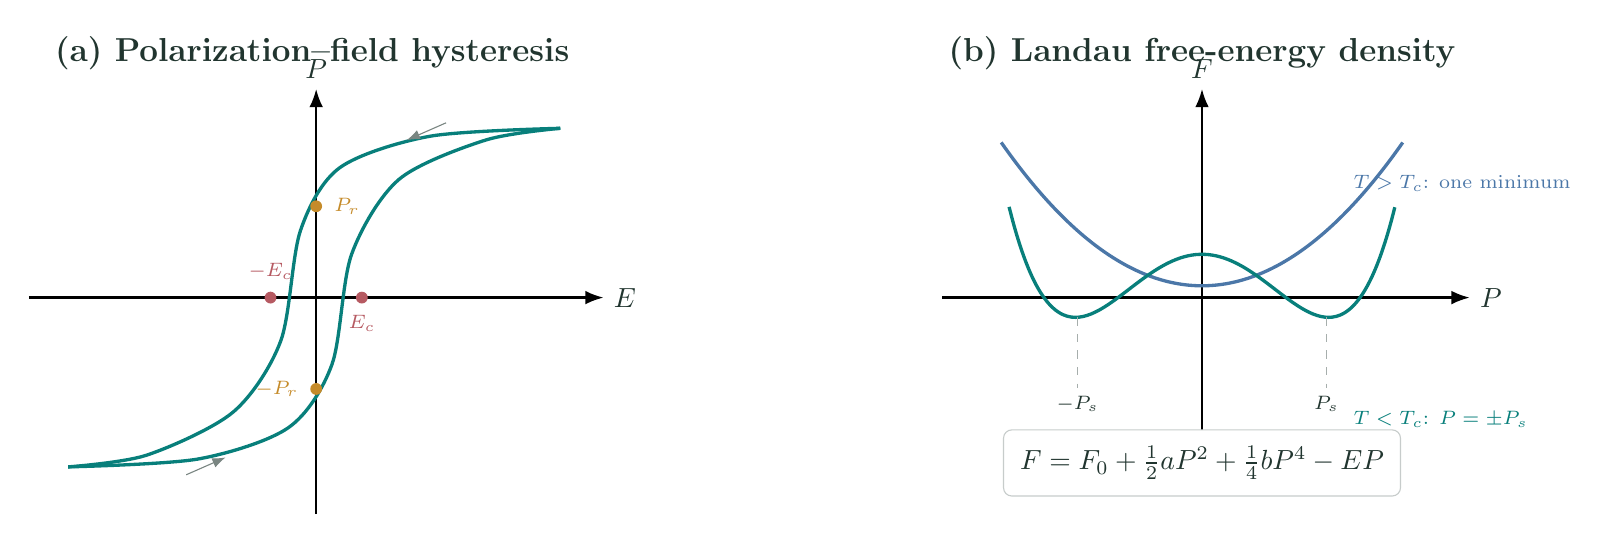
\begin{tikzpicture}[font=\sffamily,text=ink,>=Latex]
  \node[font=\bfseries\large] at (-3.4,3.1) {(a) Polarization--field hysteresis};
  \draw[->,thick] (-7.0,0)--(0.3,0) node[right] {$E$};
  \draw[->,thick] (-3.35,-2.75)--(-3.35,2.65) node[above] {$P$};
  \draw[teal,very thick] plot[smooth] coordinates {(-6.5,-2.15)(-5.5,-2.0)(-4.4,-1.45)(-3.8,-0.55)(-3.55,0.85)(-3.05,1.65)(-1.9,2.05)(-0.25,2.15)};
  \draw[teal,very thick] plot[smooth] coordinates {(-0.25,2.15)(-1.2,2.0)(-2.3,1.5)(-2.9,0.55)(-3.15,-0.85)(-3.7,-1.65)(-4.85,-2.05)(-6.5,-2.15)};
  \fill[gold] (-3.35,1.16) circle (0.075) node[right=3pt,font=\scriptsize] {$P_r$};
  \fill[gold] (-3.35,-1.16) circle (0.075) node[left=3pt,font=\scriptsize] {$-P_r$};
  \fill[rose] (-2.77,0) circle (0.075) node[below=3pt,font=\scriptsize] {$E_c$};
  \fill[rose] (-3.93,0) circle (0.075) node[above=3pt,font=\scriptsize] {$-E_c$};
  \draw[->,ink!60] (-5.0,-2.25)--(-4.5,-2.03);
  \draw[->,ink!60] (-1.7,2.22)--(-2.2,2.00);

  \begin{scope}[xshift=4.7cm]
    \node[font=\bfseries\large] at (3.2,3.1) {(b) Landau free-energy density};
    \draw[->,thick] (-0.1,0)--(6.6,0) node[right] {$P$};
    \draw[->,thick] (3.2,-2.5)--(3.2,2.65) node[above] {$F$};
    \draw[blue,very thick,domain=-2.55:2.55,samples=90,smooth,variable=\x] plot ({3.2+\x},{0.28*\x*\x+0.15});
    \node[blue,anchor=west,font=\scriptsize] at (5.0,1.45) {$T>T_c$: one minimum};
    \draw[teal,very thick,domain=-2.45:2.45,samples=100,smooth,variable=\x] plot ({3.2+\x},{0.12*\x*\x*\x*\x-0.62*\x*\x+0.55});
    \node[teal,anchor=west,font=\scriptsize] at (5.0,-1.55) {$T<T_c$: $P=\pm P_s$};
    \draw[dashed,ink!40] (1.62,-0.25)--(1.62,-1.15);
    \draw[dashed,ink!40] (4.78,-0.25)--(4.78,-1.15);
    \node[font=\scriptsize] at (1.62,-1.35) {$-P_s$};
    \node[font=\scriptsize] at (4.78,-1.35) {$P_s$};
    \node[draw=ink!25,rounded corners=3pt,inner sep=6pt,fill=white] at (3.2,-2.1) {$F=F_0+\frac12aP^2+\frac14bP^4-EP$};
  \end{scope}
\end{tikzpicture}
\end{document}
